\documentclass{standalone}
\usepackage{tikz}
\usepackage{ctex,siunitx}
\setCJKmainfont{Noto Serif CJK SC}
\usepackage{tkz-euclide}
\usepackage{amsmath,upgreek}
\usetikzlibrary{patterns, calc,3d}
\usetikzlibrary {decorations.pathmorphing,decorations.pathreplacing,decorations.shapes}
\begin{document}
\small
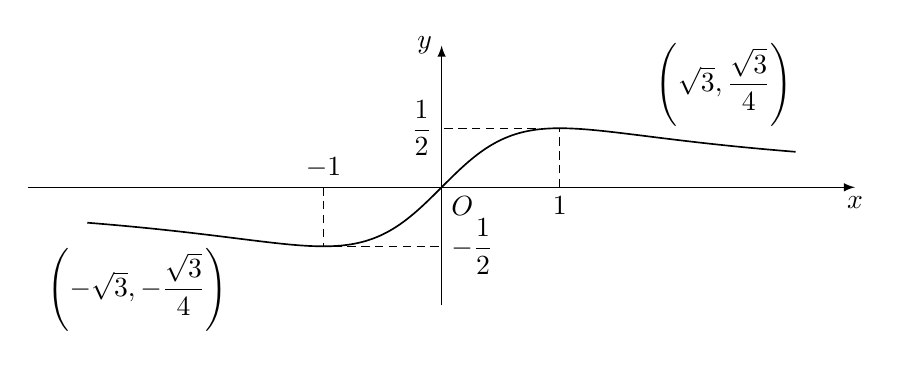
\begin{tikzpicture}[>=latex,scale=1.5]
  \draw[->](-3.5,0)--(3.5,0)node[below]{$x$};
  \draw[->](0,-1)--(0,1.2)node[left]{$y$};
  \node at (0,0)[below right]{$O$};
  \draw[samples=200,domain=-3:3,semithick]plot(\x,{\x/(1+\x*\x)});
  \draw[densely dashed](-1,0)node[above]{$-1$}--(-1,-0.5)--(0,-0.5)node[right]{$-\dfrac12$};
  \draw[densely dashed](1,0)node[below]{$1$}--(1,0.5)--(0,0.5)node[left]{$\dfrac12$};
  \node at ({sqrt(3)},{0.25*sqrt(3)})[above right]{$\left(\sqrt{3},\dfrac{\sqrt{3}}{4}\right)$};
  \node at ({-sqrt(3)},{-0.25*sqrt(3)})[below left]{$\left(-\sqrt{3},-\dfrac{\sqrt{3}}{4}\right)$};
\end{tikzpicture}
\end{document}